\documentclass{scrbook}
\usepackage{graphicx} % Required for inserting images
\usepackage{tabularx} % Required for fixed width tables
\usepackage{scrlayer-scrpage} % Required for the subtitles
\usepackage{url} % Required for the URLs
\usepackage{hyperref} % Required for the URLs
\usepackage{listings} % Required for the code snippets
\usepackage{mathtools} % Required for the system of equations
\usepackage{amsmath,amssymb} % Required for some math symbols
\usepackage{enumitem} % Required for lettered lists

% Put the caption of the snippets at the bottom
\lstset{
    captionpos=b
}


\title{Blockchain consensus protocols}
\subtitle{Ambient intelligence course (A.Y. 2025/2026)\\Topic taught by Prof. Arnaldo Tomasino}
\author{Gabriele Colapinto}
\date{\today}

\begin{document}

\maketitle
\thispagestyle{empty}

{\Large\textbf{License}} \\
{Notes from Ambient intelligence (A.Y. 2025/2026) by Gabriele Colapinto. 
Course taught by professors Michele Ruta, Floriano Scioscia, Arnaldo Tomasino, Davide Loconte — 
Licensed under CC BY-NC 4.0.\\
\url{https://creativecommons.org/licenses/by-nc/4.0/}}

\vspace*{\fill}
\rule{\textwidth}{0.2pt}
\small{© 2025 Gabriele Colapinto \\
Released under the \href{https://creativecommons.org/licenses/by-nc/4.0/}{Creative Commons Attribution–NonCommercial 4.0 International License}}

\clearpage

\tableofcontents

\chapter{Introduction to Blockchain Consensus Protocols}

\begin{figure}[htbp]
    \centering
    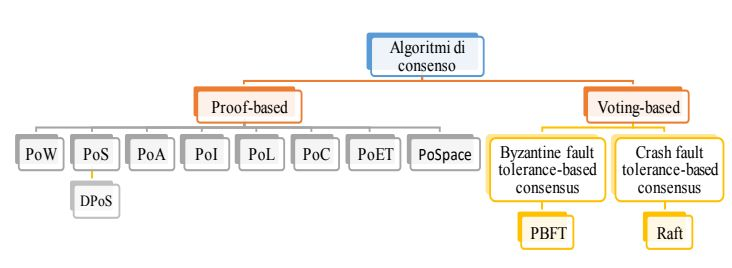
\includegraphics[width=\linewidth]{Images/Consensus_protocol_classification.jpg}
    \caption{Consensus protocols classification}
    \label{fig:consensus_protocols_classification}
\end{figure}

Consensus protocols are the set of rules and procedures that allow a distributed network of independent computers, or nodes, to agree on a single, shared state of the ledger. These mechanisms are the cornerstone of a blockchain's security and integrity, as they ensure that every node maintains an identical copy of the transaction history, even in the presence of network faults or malicious actors attempting to disrupt the system. Without a robust consensus protocol, a decentralized network would be unable to maintain trust among its participants. \\

Consensus algorithms can be broadly categorized along two primary dimensions (See figure ~\ref{fig:consensus_protocols_classification_graph}):

\begin{figure}
    \centering
    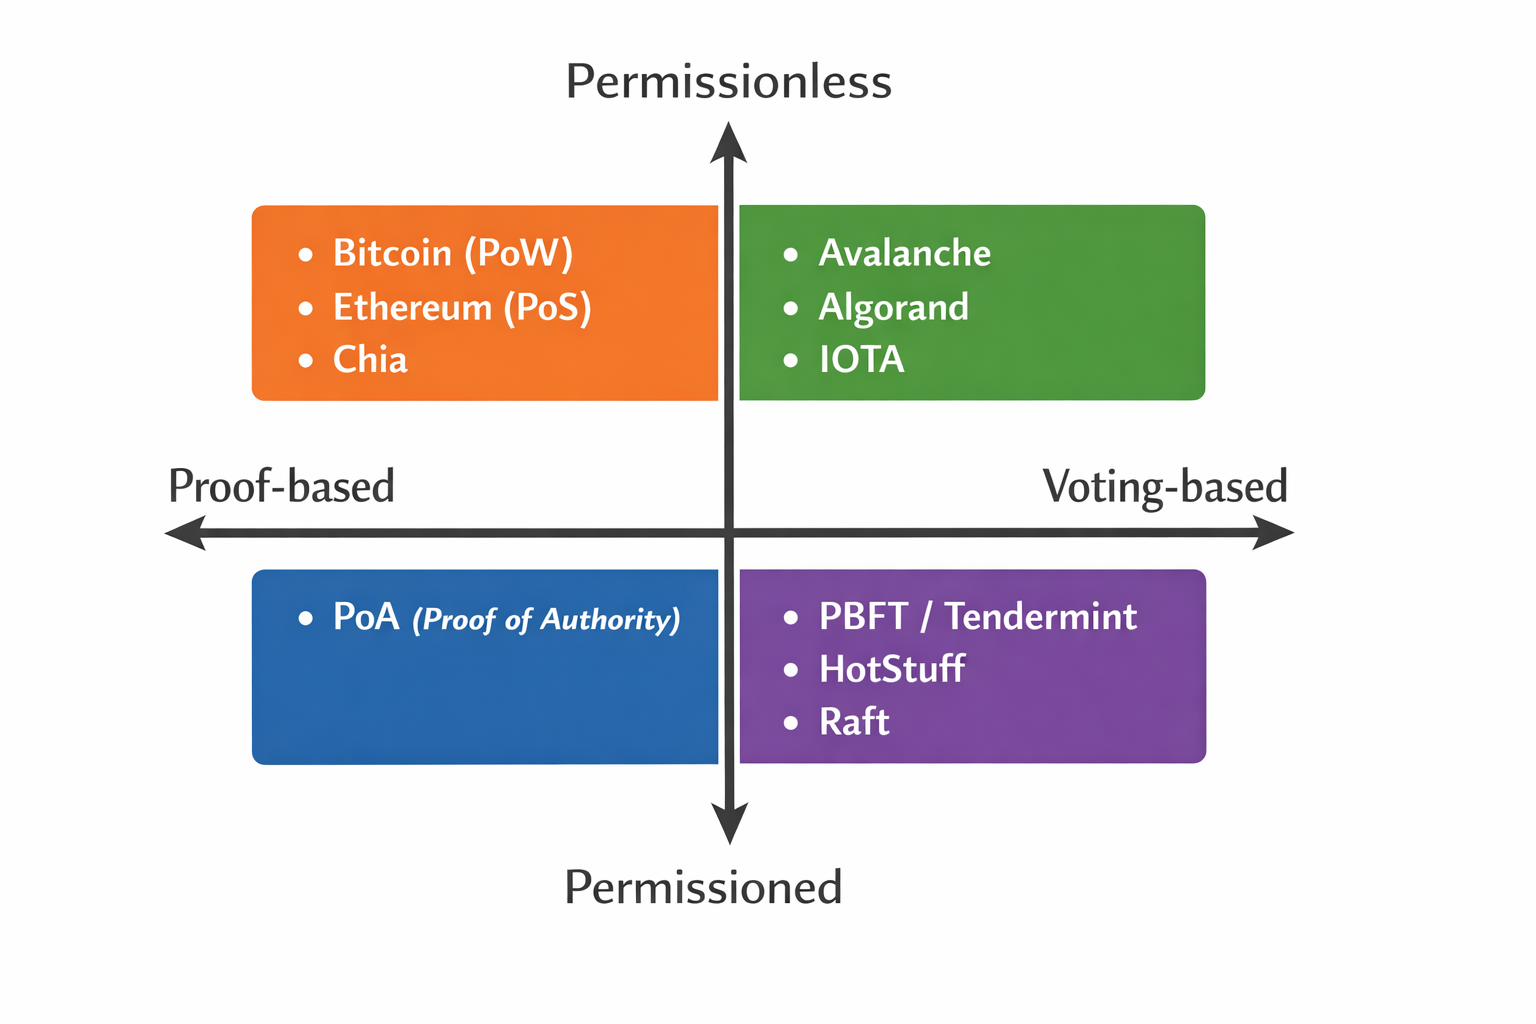
\includegraphics[width=0.8\linewidth]{Images/Consensus_protocol_classification_graph.png}
    \caption{Consensus protocol classification graph}
    \label{fig:consensus_protocols_classification_graph}
\end{figure}

\begin{enumerate}
    \item \textbf{Proof-based vs. Voting-based:} Proof-based algorithms require participants to demonstrate a verifiable commitment of a scarce resource (like computing power or capital) to participate. Voting-based algorithms, by contrast, rely on a set of known participants reaching a formal agreement through a voting process.
    \item \textbf{Permissionless vs. Permissioned:} This classification refers to the network's access control model, which fundamentally shapes the design of its consensus protocol.
\end{enumerate}

Table ~\ref{tbl:permissionless_vs_permissioned_blockchains} contrasts these two architectural models. \\

\begin{table}[htbp]
    \centering
    \begin{tabular}{|p{0.2\textwidth}|p{0.35\textwidth}|p{0.35\textwidth}|}
    \hline
    \textbf{Characteristic} & \textbf{Permissionless Blockchain} & \textbf{Permissioned Blockchain} \\
    \hline
    \textbf{Access Control} & Anyone can join the network to read, write, and participate in consensus without prior authorization. & Only authorized parties can join the network and participate in the consensus protocol. \\
    \hline
    \textbf{Participant Identity} & Participants can be anonymous or pseudonymous. Identity is not a prerequisite for participation. & Participants are known, and their identities must be authenticated to join the network. \\
    \hline
    \textbf{Consensus Robustness} & Must be highly robust to defend against attacks from unknown and potentially malicious actors (e.g., Sybil attacks). & Can use less computationally intensive protocols, as the set of participants is known and trusted to a degree. \\
    \hline
    \textbf{Incentive Model} & Participants are typically rewarded with a native cryptocurrency for their contributions to securing the network. & Incentives may not be required, as participants are often organizations with a vested interest in the network's operation. \\
    \hline
    \textbf{Example Platforms} & Bitcoin, Ethereum & Hyperledger Fabric \\
    \hline
    \end{tabular}
    \caption{Permissionless vs. Permissioned Blockchains}
    \label{tbl:permissionless_vs_permissioned_blockchains}
\end{table}

The most foundational and widely recognized consensus protocol, particularly in permissionless systems, is Proof of Work.

\chapter{Proof-Based Protocols: Verifiable Effort and Resource Commitment}

Proof-based protocols are a class of consensus algorithms that require participants—often called miners or validators—to demonstrate a verifiable commitment of a specific, costly resource. This "proof" serves as a ticket to participate in the consensus process, such as proposing a new block. The resource committed can be computational power, capital (cryptocurrency), disk storage, or even elapsed time. The underlying principle is that by making participation costly, the protocol can deter malicious activity and secure the network.

\section{Proof of Work (PoW)}

\subsection{Definition}

Proof of Work (PoW) is a protocol designed primarily to prevent Sybil attacks, where an attacker creates numerous pseudonymous identities to gain a disproportionate influence over the network. PoW makes the creation of new blocks computationally difficult and therefore expensive, linking block creation rights to real-world economic resources.

\subsection{Core mechanism}

Network participants, known as \textit{miners}, compete to solve a difficult cryptographic challenge. This involves repeatedly hashing the block's header data with different values for a random number called a \texttt{nonce} which is part of the block header (See figure ~\ref{fig:block_header}). The goal is to find a \texttt{nonce} that results in a \texttt{SHA-256} hash that is numerically below a given target value (See figure ~\ref{fig:pow_hash_computation}). In practice, this is equivalent to finding a hash that starts with a required number of leading zeros.

\begin{center}
    $Block \, Hash \leq T \, (target \, value) \Leftrightarrow It \, starts \, with \, n \, zeroes$
\end{center}

Let us expose how the number of leading zeroes $n$ influences the difficulty. The hashing function \texttt{SHA-256} has a fixed output length of $256$ bits. Hashing functions are non-invertible meaning that one can't start from a target value an derive the \texttt{nonce} that solves the challenge analytically. This means that the nonce is to be guessed by the miners. When a miner tries a random nonce value, they cannot know in advance the result of the hashing function meaning that, to the eyes of the miner, the result of the hashing function is a random sequence of bits. At this point the chances of finding a valid nonce are proportionate to the size of the range of the output value. Until now, we have considered the number of leading zeroes $n$. But let us look at the result of the hashing function from the other side. The number of bits of the target value (labeled with an $X$ in figure ~\ref{fig:pow_hash_computation}) is:

\begin{center}
    $n_X \; (Target \; value \; bits) = 256 \; (Total \; number \; of \; bits) - n \; (Leading \; zeros)$
\end{center}

\newpage

The greater the value of $n$ the smaller the range for the target value. For example:

\begin{table}[htbp]
\centering
    \begin{tabular}{l l}
        $For \; n=10:$ & $n_X = 256 - n = 246 \; bits \Rightarrow 2^{246} \; possible \; valid \; values$ \\
        $For \; n=100:$ & $n_X = 256 - n = 156 \; bits \Rightarrow 2^{156} \; possible \; valid \; values$ \\
    \end{tabular}
\end{table}

Let us make a metaphor to better understand the concept: let's say that we are blindfolded and we want to throw a ball in a basket in front of us. Doing so in a small basket is more difficult than doing it in a bigger basket. Increasing $n$ decreases $n_X$ reducing the size of the basket. Conversely, decreasing $n$ increases $n_X$ increasing the size of the basket. \\

\texttt{Increasing $T$ decreases $n$ and the difficulty of the challenge while decreasing $T$ increases $n$ and the difficulty of the challenge.} 

\subsection{Difficulty Adjustment in Bitcoin Proof of Work}

The Bitcoin protocol is designed to keep the average block generation time approximately constant (about 10 minutes), independently of the total amount of computational power available in the network. This goal is achieved through an automatic \emph{difficulty adjustment} mechanism for the cryptographic challenge.

\paragraph{Why the difficulty must change}

Satoshi Nakamoto knew that people would have seen bitcoin mining as a profitable activity and expected many people to join the network as miners and the technology to evolve to mine more efficiently. Think about it: miners want the mining task to become simpler in order to employ less resources to get value thus increasing their profit. Considering that both people joining the network and technology advancement increase the number of hashes generated in a given time unit we say that those activities increase the network \textbf{hashrate}. \\

If the difficulty were kept constant:

\begin{itemize}
    \item an increase in the total network hashrate would cause blocks to be found too quickly;
    \item a decrease in hashrate would make the blockchain extremely slow.
\end{itemize}

To prevent these effects, every 2016 blocks the protocol compares the actual time required to generate them with the expected time ($2016 \times 10$ minutes) and updates the difficulty deterministically:

\begin{itemize}
    \item if blocks are found too quickly, the difficulty is increased;
    \item if blocks are found too slowly, the difficulty is decreased.
\end{itemize}

This mechanism implements a simple distributed feedback control system.

\paragraph{How a single miner perceives difficulty}

From the perspective of an individual miner, the difficulty does not change the mining procedure itself: the miner continues to compute hashes by varying the nonce and attempting to find a valid one. What changes is the \emph{probability of success per hash}.
When the difficulty increases:

\begin{itemize}
    \item each hash has a lower probability of being valid;
    \item the expected time to find a block (or a share) increases;
    \item the expected revenue per unit of time decreases, given a fixed hashrate.
\end{itemize}

Thus, miners do not perceive difficulty as an operational parameter, but rather as a statistical reduction in the frequency of successful outcomes.

\paragraph{Difficulty, economic incentives, and ASIC investment}

Difficulty directly influences the economic incentives of mining. When the total network hashrate grows, difficulty increases and mining becomes less profitable per unit of computational power.
This creates competitive pressure:

\begin{itemize}
    \item less efficient miners may be pushed out of the market;
    \item remaining miners are incentivized to invest in more efficient hardware (ASICs)
    in order to reduce the cost per hash;
    \item the system tends toward an equilibrium in which the marginal cost of mining
    approaches the value of the block reward.
\end{itemize}

Investment in ASICs is therefore not a direct reaction to difficulty itself, but to the economic competition that difficulty makes explicit.

\paragraph{The lottery ticket metaphor}

A useful intuitive model for Proof of Work is the lottery metaphor:

\begin{itemize}
    \item each hash computed by a miner corresponds to buying a lottery ticket;
    \item a ticket is winning if its number is below the target;
    \item difficulty determines how rare winning tickets are.
\end{itemize}

Increasing computational power is equivalent to buying more tickets per second. When too many tickets win too quickly, the protocol makes winning tickets rarer by increasing the difficulty. In this way, regardless of the number of participants or tickets purchased, the frequency of wins remains stable over time.

\paragraph{How does the network change the difficulty of the challenge?}

Bitcoin adjusts the target every 2016 blocks to keep the block generation rate $r$ approximately equal to 10 minutes.  Ideally, $r \cdot 2016 = 10 \; min \; \cdot 2016 = 2 \; weeks$ so, the difficulty of the challenge is updated every 2 weeks. \\

To update the difficulty of the challenge we need to know if the old threshold value made the challenge easier or harder than intended. We get this information by considering the actual time elapsed to mine the 2016 block and comparing it with the ideal time of 2 weeks (all in minutes). We call $f$ the ratio between the actual time and the intended time:

\begin{center}
    $f = \frac{t_{actual}}{2016 \; \cdot \; 10 \; min}$
\end{center}

We use $f$ and the previous target value $T_{prev}$ to calculate the new target value $T$ as follows:

\begin{center}
    \[
        T =
        \begin{cases}
            \frac{T_{prev}}{4} \quad f \leq 1/4 \\
            f\cdot T_{prev} \quad 1/4 < f \leq 4 \\
            4 \cdot T_{prev} \quad f \geq 4
        \end{cases}
    \]
\end{center}

\subsection{Security assumption}

The fundamental security assumption of PoW is that the blockchain remains secure as long as the majority of the network's computing power is controlled by honest nodes who follow the protocol's rules.

\subsection{Drawbacks}

The most significant criticism of Proof of Work is its extremely high energy consumption, a direct consequence of the immense computational effort required from miners worldwide. The energy consumption problem led many miners to move to China for the lower electricity cost. This created pools of miners which, in turn, generated an additional problem. Mining in pools (basically joining forces) makes mining more efficient but this goes against the decentralization principle which is the foundation of distributed platforms. \\

Nowadays, 8 pools currently account for 75\% of Bitcoin generated blocks. (See figure ~\ref{fig:mining_pools}) \\

The presence of mining pools also exposes the network to \textbf{eclipse attacks} which are attacks to a specific set of nodes. If a big set of nodes is in the same place, disrupting or isolating a set of nodes becomes simpler.

\begin{figure}
    \centering
    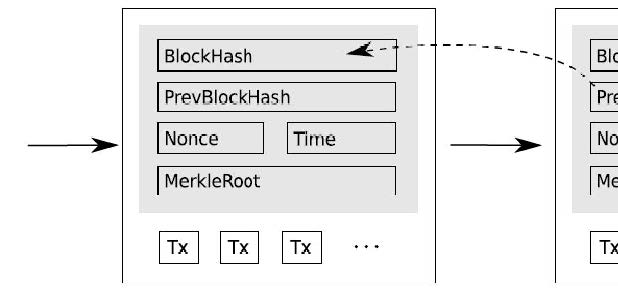
\includegraphics[width=0.5\linewidth]{Images/Block_header.jpg}
    \caption{Block header}
    \label{fig:block_header}
\end{figure}

\begin{figure}
    \centering
    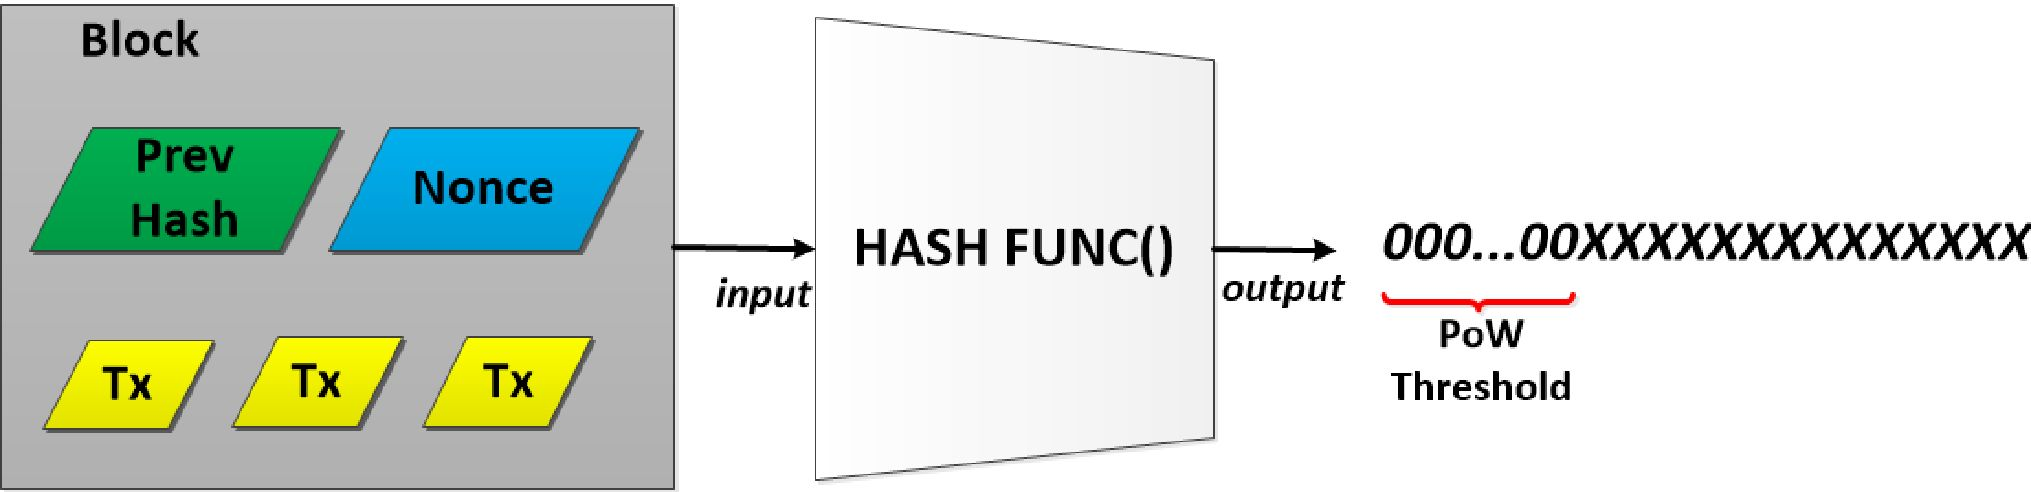
\includegraphics[width=\linewidth]{Images/Hash_computation.jpg}
    \caption{PoW hash computation}
    \label{fig:pow_hash_computation}
\end{figure}

\begin{figure}
    \centering
    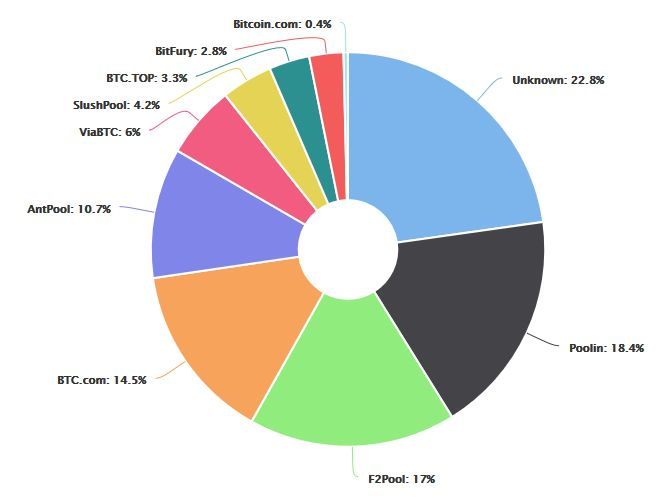
\includegraphics[width=0.5\linewidth]{Images/Mining_pools.jpg}
    \caption{Mining pools}
    \label{fig:mining_pools}
\end{figure}

\section{Proof of Stake (PoS)}

\begin{enumerate}
    \item \textbf{Definition:} Proof of Stake (PoS) has emerged as a leading, energy-efficient alternative to PoW. It replaces the competition based on computational power with one based on capital commitment.
    \item \textbf{Core Mechanism:} In PoS systems, participants known as \textit{validators} are selected to create new blocks based on the quantity of the network's native cryptocurrency they are willing to "stake" as collateral. By locking up their own funds, validators are economically incentivized to act honestly, as malicious behavior could result in them losing their staked capital (a penalty known as "slashing").
    \item \textbf{Key Variants:} Several variations of PoS have been developed to address different design goals and security considerations:
    \begin{itemize}
        \item \textbf{Delegated Proof of Stake (DPoS):} In this model, token holders use their stake to vote for a limited number of delegates (also called "witnesses"). These elected delegates are then responsible for validating transactions and producing blocks on behalf of the network.
        \item \textbf{Nominated Proof of Stake (NPoS):} This variant involves the election of a committee of validators who then take turns producing blocks in a randomized fashion, sharing the responsibility of maintaining the network.
        \item \textbf{Liquid Proof of Stake (LPoS):} This model allows token holders to delegate their staking rights to other validators without transferring custody of their tokens. This creates a competitive market for validation services and allows smaller token holders to participate in securing the network.
    \end{itemize}
    \item \textbf{Vulnerabilities:} Historically, early PoS designs were susceptible to specific vulnerabilities, such as the \textbf{"Nothing at Stake"} problem (where validators have no disincentive to support multiple conflicting chains) and \textbf{"Long-Range Attacks"} (where an attacker could potentially rewrite a large portion of the blockchain's history). Modern PoS protocols have developed mechanisms to mitigate these risks.
\end{enumerate}


\section{Other Proof-Based Models}

Beyond PoW and PoS, several other novel proof-based consensus models have been proposed, each leveraging a different resource as the basis for network security. \\

These proof-based systems contrast with protocols that rely not on individual proofs of commitment but on collective agreement among a known group of actors.

\chapter{Voting-Based Protocols: Reaching a Quorum}

Voting-based consensus protocols operate on the principle of collective agreement. These mechanisms are primarily employed in permissioned blockchains, where the participants are known and have been granted authorization to join the network. Instead of competing to solve a puzzle, a group of nodes must explicitly vote to reach an agreement, or quorum, on the validity and order of transactions to be added to the ledger.

\section{Practical Byzantine Fault Tolerance (PBFT)}

Practical Byzantine Fault Tolerance (PBFT) is a consensus algorithm designed to achieve
\emph{state machine replication} in asynchronous distributed systems in the presence of
Byzantine faults. The algorithm guarantees safety and liveness provided that at most
$f$ replicas are faulty, assuming a total of $|R| = 3f + 1$ replicas.

PBFT is a \emph{permissioned} and \emph{voting-based} consensus algorithm: the set of
participating replicas is fixed and known in advance, and consensus is reached through
explicit message exchanges rather than cryptographic proofs such as Proof of Work.

\subsection{Client Request and System Model}

The PBFT protocol operates on \emph{client requests}, which represent application-level
operations to be executed by the replicated service. A client request has the form:
\[
\langle \text{operation}, \text{timestamp}, \text{client\_id} \rangle
\]
and is digitally signed by the client to ensure authenticity.

It is important to emphasize that the client request \emph{does not} contain a new
version of the blockchain or a freshly mined block. PBFT was originally designed for
state machine replication, not for mining-based blockchains. The client merely submits
an operation to be ordered and executed consistently by all correct replicas. \\

The client sends the request to the \emph{primary replica} (leader) of the current view. (See figure ~\ref{fig:pbft_client_request})

\begin{figure}
    \centering
    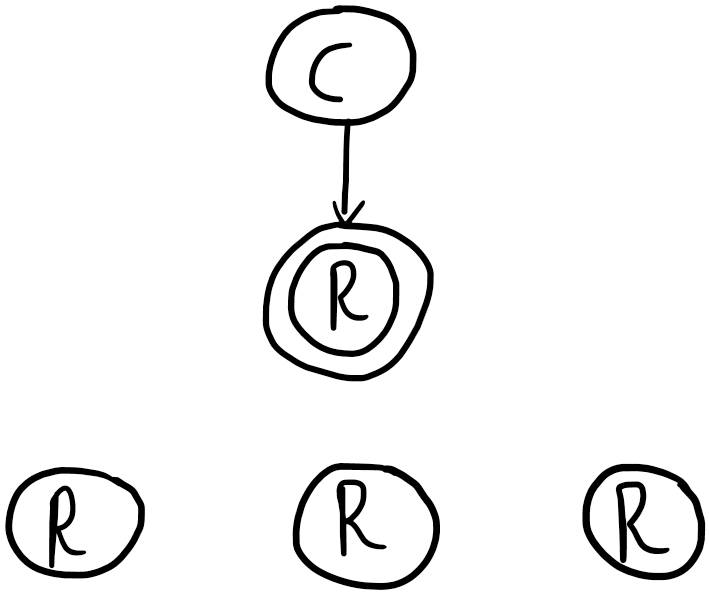
\includegraphics[width=0.5\linewidth]{Images/PBFT_client_request.png}
    \caption{PBFT client request}
    \label{fig:pbft_client_request}
\end{figure}

\subsection{Multi-Phase Communication in PBFT}

To reach agreement on the execution order of a client request, PBFT uses a three-phase
protocol:
\begin{enumerate}
    \item Pre-prepare
    \item Prepare
    \item Commit
\end{enumerate}

Each phase contributes to ensuring agreement and preventing equivocation by faulty replicas.

\subsubsection{Pre-Prepare Phase}

In the pre-prepare phase, the primary replica assigns a sequence number to the client
request and broadcasts a \texttt{PRE-PREPARE} message to all other replicas (See figure ~\ref{fig:pbft_pre-prepare_phase}):
\[
\text{PRE-PREPARE} =\langle \text{view}, \text{seq}, \text{digest(request)} \rangle
\]

The message contains:
\begin{itemize}
    \item the current view number,
    \item a sequence number defining the total order,
    \item a cryptographic digest of the client request.
\end{itemize}

Replicas verify the validity of the message and the correspondence between the digest
and the received request. At this stage, the primary is proposing \emph{what} to execute
and \emph{in which order}, but no agreement has yet been reached.

\begin{figure}
    \centering
    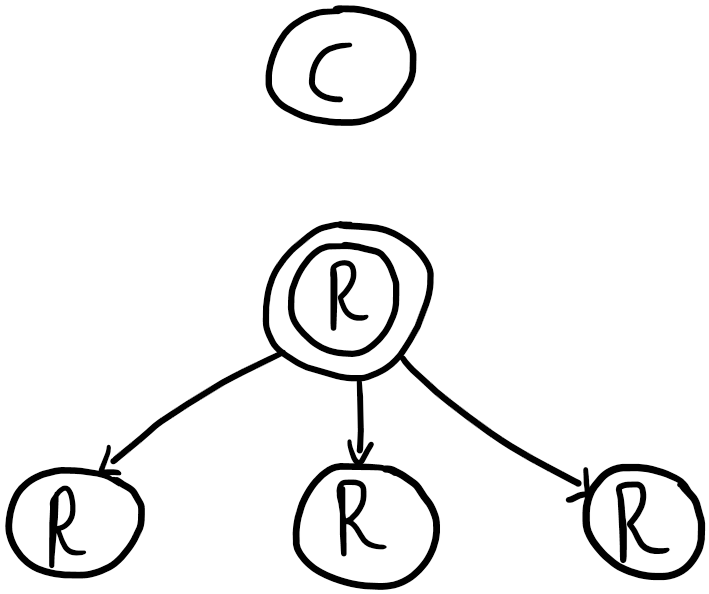
\includegraphics[width=0.5\linewidth]{Images/PBFT_pre-prepare_phase.png}
    \caption{PBFT pre-prepare phase}
    \label{fig:pbft_pre-prepare_phase}
\end{figure}

\subsubsection{Prepare Phase}

Upon accepting a pre-prepare message, a replica broadcasts a \texttt{PREPARE} message to
all other replicas (See figure ~\ref{fig:pbft_broadcast}):
\[
\text{PREPARE} = \langle \text{view}, \text{seq}, \text{digest(request)}, \text{replica\_id} \rangle
\]

A replica considers a request \emph{prepared} when it has received:
\begin{itemize}
    \item the corresponding pre-prepare message, and
    \item $2f$ matching prepare messages from distinct replicas.
\end{itemize}

This phase ensures that a quorum of replicas agrees on both the content and the ordering
of the request, preventing a faulty primary from proposing conflicting values.

\begin{figure}
    \centering
    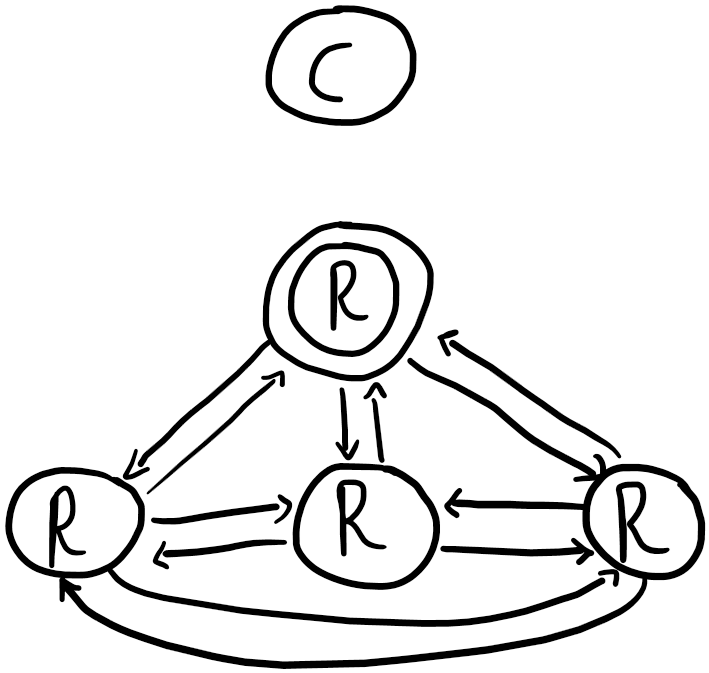
\includegraphics[width=0.5\linewidth]{Images/PBFT_prepare_phase.png}
    \caption{PBFT replicas broadcast messages used in the prepare and in the commit phases}
    \label{fig:pbft_broadcast}
\end{figure}

\subsubsection{Commit Phase}

Once a request is prepared, replicas broadcast a \texttt{COMMIT} message (See figure ~\ref{fig:pbft_broadcast}):
\[
\text{COMMIT} = \langle \text{view}, \text{seq}, \text{digest(request)}, \text{replica\_id} \rangle
\]

A request is considered \emph{committed} when a replica receives $2f + 1$ matching commit
messages. Only after this condition is met does the replica execute the operation.
The commit phase guarantees \emph{irreversibility}: once a request is committed, no
conflicting request can be decided for the same sequence number.

\subsection{Execution and Client Reply}

After executing the committed operation, each replica sends a \texttt{REPLY} message to
the client (See figure ~\ref{fig:pbft_reply}). The client waits for $f + 1$ matching replies, ensuring that at least one
reply originates from a correct replica.

\begin{figure}
    \centering
    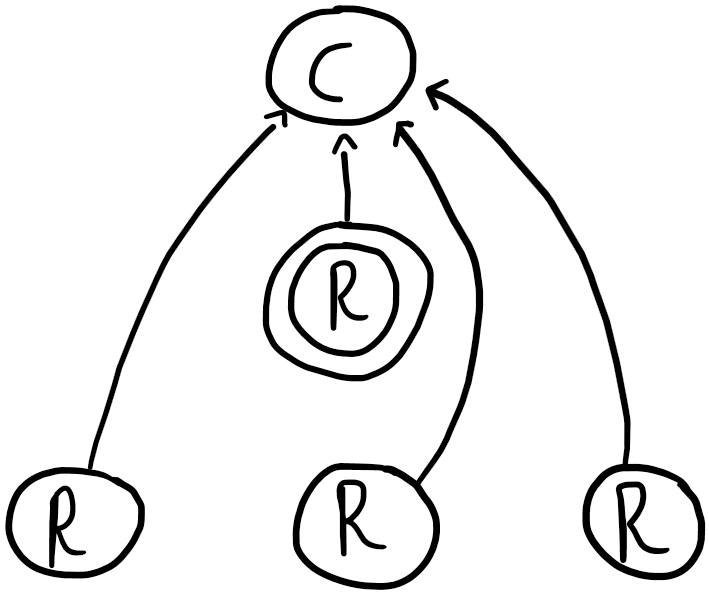
\includegraphics[width=0.5\linewidth]{Images/PBFT_reply.png}
    \caption{PBFT reply messages from the replicas to the client}
    \label{fig:pbft_reply}
\end{figure}

\subsection{PBFT in the Context of Blockchains}

Although PBFT was not originally designed for blockchains, it is widely used as a
building block in permissioned blockchain systems such as Tendermint, Hyperledger
Fabric, and HotStuff-based protocols.

In a blockchain context:
\begin{itemize}
    \item the client request typically represents a transaction or smart contract invocation;
    \item blocks are proposed by designated replicas (proposers), not by clients;
    \item PBFT phases are used to agree on the validity and ordering of blocks.
\end{itemize}

Conceptually, the PBFT phases map to blockchain operations as follows:
\begin{itemize}
    \item \textbf{Pre-prepare}: proposal of a candidate block;
    \item \textbf{Prepare}: voting on the proposed block;
    \item \textbf{Commit}: finalization of the block;
    \item \textbf{Execution}: appending the block to the local blockchain.
\end{itemize}

Therefore, contrary to mining-based blockchains, block creation and finality in PBFT-based
systems arise from coordinated voting among known validators rather than from solving
cryptographic puzzles.

\subsection{Clarification of Common Misconceptions}

To summarize:
\begin{itemize}
    \item the client does not submit a block or a blockchain state;
    \item PBFT orders and executes operations, not mined blocks;
    \item block structures are an application-layer abstraction built on top of PBFT.
\end{itemize}

This distinction is essential to correctly understand the role of PBFT in modern permissioned blockchain architectures.

\section{Raft}

\begin{enumerate}
    \item \textbf{Definition:} Raft is a consensus algorithm designed with understandability as a primary goal. Its main purpose is to manage a replicated log in a distributed system, ensuring that all nodes maintain an identical sequence of entries.
    \item \textbf{Crucial Limitation:} It is essential to note that Raft is \textbf{not} Byzantine Fault Tolerant. It operates under the assumption that nodes may fail (e.g., crash or have network issues) but are not malicious. The protocol relies on nodes trusting the elected leader.
    \item \textbf{Core Mechanism:} The system is leader-based. A single \texttt{leader} is elected from among the nodes and is solely responsible for accepting client requests and replicating log entries to the other \texttt{follower} nodes. If the leader fails or becomes unresponsive, the follower nodes will time out and initiate a new election to choose a new leader.
    \item \textbf{Common Use Cases:} Due to its simplicity and fault-tolerant (but not Byzantine-tolerant) nature, Raft is widely used for managing state and configuration in permissioned distributed systems such as the etcd distributed key-value store and the CockroachDB distributed SQL database.
\end{enumerate}

The choice of data structures and a consensus protocol is not an arbitrary design decision. It is a fundamental choice that defines a blockchain's core characteristics, shaping its security model, transaction throughput, degree of decentralization, energy efficiency, and overall governance structure. Understanding these components is therefore essential to evaluating and engineering any blockchain system.

\end{document}
